\chapter{Evaluation\label{chap:evaluation}}
  This chapter will detail the evaluation metrics, how they were used to test the performance of the tool and what the results of the evaluation were. Two studies were carried out making use of six debates from our corpus \cite{walker2012corpus}: abortion, creation, gay rights, the existence of god, gun ownership and healthcare. A final study was carried out making use of the same debate summaries and two new summaries for discussion on Twitter around the 2014 Independence Referendum.

  \section{Research Questions}
    We wanted to evaluate our tool as an automatic summarization tool. The result of a final analysis stage was a summary comprising of point extracts for a given debate, by assessing the quality of this we can also evaluate the precursor points extraction analysis. The following research questions were set:

    \begin{itemize}
      \item{Are our summaries more readable and informative than those produced by existing tools?}
      \item{Does introducing summary sections with an explanation improve readability?}
      \item{How well does our bigram-based extract selection perform?}
      \item{Which sections of generated summaries are most and least useful to readers?}
    \end{itemize}

    To address these questions we compared different versions of our summaries against equal-length summaries generated by an implementation \footnote{http://homepages.abdn.ac.uk/advaith/pages/teaching/NLP/practicals/Practical3.zip} of the approach described by Nenkova et al. \cite{nenkova2006compositional}. We also gathered scores for groups of extracts allocated by the bigram model for comparison with human scores. Additionally, summaries generated with randomly selected extracts against were compared against one based on our bigram model for selection.

  \section{Design}
    In response to the our research questions we set the following null hypotheses for the evaluation:

    \begin{itemize}
      \item{The readability and informativeness of our summaries do not improve on those of existing tools. (\textbf{H1})}
      \item{Explanations introducing summary sections does not improve readability. (\textbf{H2})}
      \item{Our means of selecting extracts is not better than random selection. (\textbf{H3})}
      \item{All summary sections are equally useful to readers. (\textbf{H4})}
    \end{itemize}

    \tocless\subsection{Study Participants}
      To test these hypotheses, we prepared three comparative studies. These are described in Sections \ref{sec:stud1} onwards. Participants for studies 1 and 2 were recruited using Amazon Mechanical Turk. In the both studies, workers were `Mechanical Turk Masters'. Study 1, comparing summaries, had 25 unique participants giving 54 responses to 6 different tasks. Study 2, rating extracts, had 27 unique participants giving 54 responses to 6 different tasks. There were 38 participants in total across both studies, each participant could not complete the same task more than once. The average worker had completed 3 tasks and had an approval rating of 98\%.

      For Study 3 we attended a workshop with social science researchers interested in using social media analysis in their work. There were 15 present and we collected written comments from 9.

    \tocless\subsection{Summary Styles}
      In the upcoming sections, reference is made to a range of summary styles used in evaluation tasks.
      \begin{itemize}
        \item{\textbf{Stock}: A summary generated using an implementation of the approach described by Nenkova et al. \cite{nenkova2006compositional}. These Stock summaries were used as a benchmark for summaries generated by our tool. There is no structure to these summaries, they are generated by selecting sentences that reference prominent words not already included in the summary. The resulting distribution of words in the summary is close to that of the input text.}
        \item{\textbf{Plain}: This is a collection of point extracts in the same style as the Stock summaries. The extracts are still grouped into sections, only this is not made clear in the presentation. Plain summaries were designed to be as close as possible to the Stock summary presentation. Plain summaries were also of equal length to the benchmark Stock summaries.}
        \item{\textbf{Layout}: A summary that has explanatory text that introduces sections. The extracts are the same as those in the Plain summary though the explanations increase the overall word count. For a fair evaluation, these are compared against a longer Stock summary..}
        \item{\textbf{Formatted}: A Layout summary with explanation keywords in bold and topic words in green. The content is the same as a Layout summary.}
      \end{itemize}

    \tocless\subsection{Study 1: Summary Comparison\label{sec:stud1}}
      In order to address \textbf{H1} and \textbf{H2} we designed a questionnaire that compared various summary styles against equal-length Stock summaries. Each questionnaire was made up of three sections. Please see Appendix \ref{app:survey-section} for an example summary section.

      The first section compared a Plain summary against a Stock summary on the same topic. Users were instructed to read both summaries and rate them relatively on the following criteria:

      \begin{itemize}
        \item{Content Interest / Informativeness}
        \item{Readability}
        \item{Punctuation \& Presentation}
        \item{Organization}
      \end{itemize}

      Finally they were asked to give an overall rating and justify their response using free text. The following section asked the same questions but instead compared a Layout summary against a Stock one - this second comparison was for a different topic. Layout summaries are longer because of the explanatory text, the Stock summary was the same length as the Layout summary and was longer than the Stock summary used in the first section. The final section compared a Layout summary with a Formatted one. The Layout summary is reused from the second section, the Formatted summary has the same content (only different formatting). There was only an overall rating and justification for the comparison in this section.

      There were six versions of the questionnaire setup in a Latin square to cover all six topics. Section 1 had a different topic from sections 2 so as to not repeat summary content. Section 3 addresses the question of formatting only and has the same content as the Layout summary in section 2 to make the task faster.

      Responses from the first section that compare our Plain summary against a Stock one can be used in addressing \textbf{H1}. The difference in the responses gathered in section 2 will allow us to address \textbf{H2}. Section 3 expands on this, testing if the formatting is a useful addition to the Layout summary.

    \tocless\subsection{Study 2: Extract Comparison}
    To investigate the performance of the tool in greater depth we ran a further study testing the quality of our extract selection mechanism. Responses from this questionnaire addressed \textbf{H3}. See Appendix \ref{app:extract-survey-section} for an example section.

    The task given to participants had two sections. First were three sets of extracts for three different point patterns, participants were asked to rate extracts accounting for their succinctness and the extent to which they made sense. This was the closest we could make the task for participants to that of the aim of the tool. The following section, similar to the first study, compared two summaries (see Appendix \ref{app:survey-section}). Both summaries were of the Formatted style however this time their content differed. The extracts in one summary were selected using the bigram model, the extracts in the other were selected at random from the same clusters of points. Participants were asked to give these a relative rating and justify their response. Responses for these two tasks were intended to address \textbf{H3}.

    \tocless\subsection{Study 3: Section Comparison}
      This study was completed as a paper exercise with workshop participants in a session before the approach was discussed. Participants were given side-by-side summary comparisons, similar to the first study, however only qualitative feedback was requested. Given two comparisons of Layout and Stock summaries on two different topics, participants were prompted to:

	  \blockquote{
        \textit{
          Write your comments about the two summaries. Feel free to
          say anything that strikes you, but particularly address:
          \begin{itemize}
            \item{Which you prefer, and why?}
            \item{Do you like the structuring into sections in one of the summaries?}
          \item{Which sections are most interesting to you?}
          \item{What other sections might be useful to you that are missing?}
          \end{itemize}
        }
      }

      Responses from this task were intended to answer to \textbf{H4}. We also introduced two new summaries: `Before Referendum' \& `Referendum Day' based on tweets referencing the \#indyref tag or mentioning one of the campaign accounts for those date ranges. One of these summaries made up the second comparison for each participant. The first comparison was selected from either: \textit{Abortion}, \textit{Gay Rights}, \textit{Existence of God} or \textit{Gun Laws}. These four were selected from the six available as they had all summary sections complete.

  \section{Results}
    \tocless\subsection{Study 1: Summary Comparison}
      This first study made comparisons between three pairs of summary types: Plain vs. Stock, Layout vs. Stock \& Layout vs. Formatted. The results of each are reported below.

      \tocless\subsubsection{Plain vs. Stock Comparison}
        \begin{figure}[h]
          \centering
          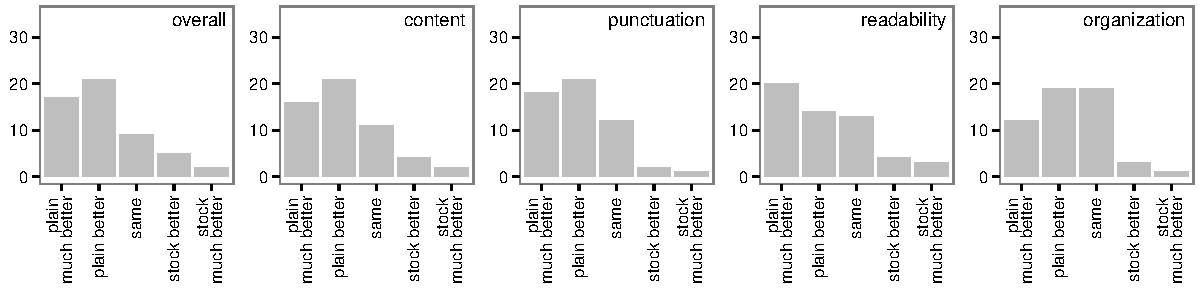
\includegraphics[width=\textwidth]{graphs/plain_vs_stock_hists}
          \caption{Counts of participant responses when comparing of Plain \& Stock.}
          \label{fig:plain_vs_stock_hist}
        \end{figure}

        \noindent All of the five comparison factors presented in \ref{fig:plain_vs_stock_hist} show a preference for our Plain summaries. These counts are aggregated from all Plain vs. Stock comparisons for the debate six topics. Each histogram represents 54 responses for a question comparing the two summary types on that factor. The results were tested using Sign tests for each comparison factor, `better' and `much better' for each type were aggregated, `same' was excluded. The family significance level was set at $\alpha = 0.05$; with $m = 5$ hypotheses - using the Bonferroni Correction ($\alpha / m$); gives an individual significance threshold as $0.05/5 = 0.01$. All factors, including `readability' \& `content', were found to show a significant difference, see Table \ref{tab:pvs-pvals}. This enables us to reject \textbf{H1} --- that our tool does not improve on existing tools --- with a good level of confidence.

		\begin{table}[h]
		  \centering
		  \caption{Plain vs. Stock factor comparison $p$ values}
		  \label{tab:pvs-pvals}
		  \begin{tabular}{|l|l|l|l|l|l|}
			\hline
			\textbf{Overall} & \textbf{Content} & \textbf{Punctuation} & \textbf{Readability} & \textbf{Organization} \\ \hline
			$p = \num{3.1e-06}$ & $p = \num{1.6e-06}$ & $p = \num{5.6e-09}$ & $p = \num{2.5e-05}$ & $p = \num{3.5e-06}$ \\ \hline
		  \end{tabular}
		\end{table}

      \tocless\subsubsection{Layout vs. Stock Comparison}

		\begin{figure}[h]
		  \centering
		  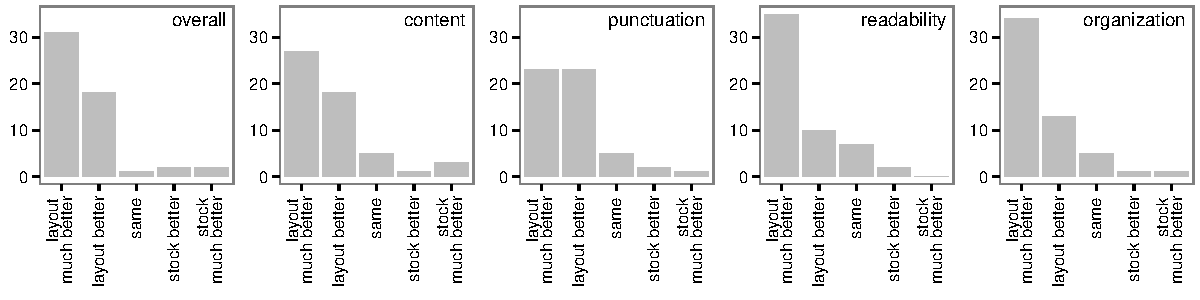
\includegraphics[width=\textwidth]{graphs/layout_vs_stock_hists}
		  \caption{Counts of participant responses when comparing of Layout \& Stock.}
		  \label{fig:layout_vs_stock_hist}
		\end{figure}

        \noindent Similarly, Layout was also compared against Stock on the same factors, the results of these comparison are presented in Figure \ref{fig:layout_vs_stock_hist}. We saw a stronger preference than in the Plain comparison. Similar to that comparison: counts are aggregated from all comparisons for all topics; each histogram represents 54 responses; comparison results were tested using Sign tests and the individual significance threshold was $0.01$. Again, all factors were found to show a significant difference for this comparison, see Table \ref{tab:lvs-pvals}. Comparing the readability scores in \ref{fig:layout_vs_stock_hist} against those in \ref{fig:plain_vs_stock_hist} shows an improvement in the readability after introducing sections to the same sets of points. \textcolor{red}{This is cause to reject \textbf{H2}. We can state that the summary sections improve readability}.

		\begin{table}[h]
		  \centering
		  \caption{Layout vs. Stock factor comparison $p$ values}
		  \label{tab:lvs-pvals}
		  \begin{tabular}{|l|l|l|l|l|l|}
			\hline
			\textbf{Overall} & \textbf{Content} & \textbf{Punctuation} & \textbf{Readability} & \textbf{Organization} \\ \hline
			$p = \num{7.1e-11}$ & $p = \num{8.2e-10}$ & $p = \num{7e-11}$ & $p = \num{1.6e-11}$ & $p = \num{4.4e-12}$ \\ \hline
		  \end{tabular}
		\end{table}

      \tocless\subsubsection{Formatted vs. Layout Comparison}
        \noindent Finally, participants compared Formatted and Layout summaries --- there was only a single `overall' factor for this comparison. Results from the 54 responses for this comparison, presented in Figure \ref{fig:lay_vs_formatted_hist}, show a preference for Formatted summaries over Layout summaries with the same content. Comparing the results again using a Sign test (aggregating `better' and `much better' and excluding `same') showed a significant result ($p = 0.006$). This result builds on the previous comparison, showing that not only sections but other elements of presentation can improve the readability of a summary.

	  \begin{figure}
		\centering
		\begin{minipage}{.25\textwidth}
		  \centering
		  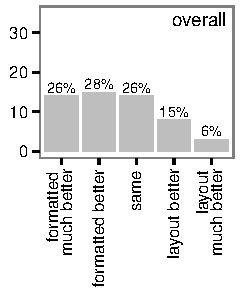
\includegraphics[width=\textwidth]{graphs/layout_vs_formatted_hists}
		  \captionsetup{width=0.95\linewidth, font={footnotesize}}
		  \captionof{figure}{Counts of participant responses when comparing of Layout \& Formatted.}
		  \label{fig:lay_vs_formatted_hist}
		\end{minipage}%
		\begin{minipage}{.5\textwidth}
		  \centering
		  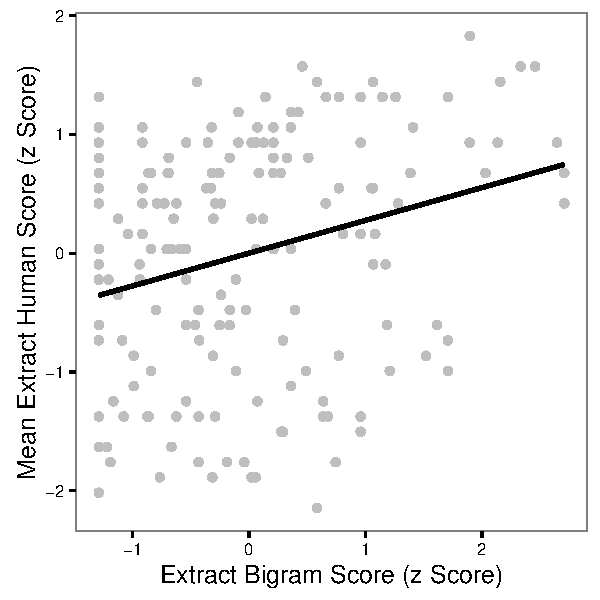
\includegraphics[width=0.8\textwidth]{graphs/scatter}
		  \captionsetup{width=0.95\linewidth, font={footnotesize}}
		  \captionof{figure}{Correlation between human and bigram standard scores.}
		  \label{fig:scatter}
		\end{minipage}%
		\begin{minipage}{.25\textwidth}
		  \centering
		  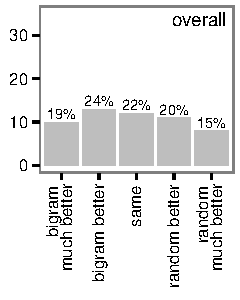
\includegraphics[width=\textwidth]{graphs/bigram_vs_random_hists}
		  \captionsetup{width=0.95\linewidth, font={footnotesize}}
		  \captionof{figure}{Counts of participant responses when comparing of Bigram \& Random.}
		  \label{fig:bigram_vs_random_hist}
		\end{minipage}%
	  \end{figure}

    \tocless\subsection{Study 2: Extract Comparison}
    Extracts selected by our tool for display were scored above average 73\% of the time. Participants were instructed to score better extracts higher on a 5-point Likert scale. Extracts selected by the bigram model scored, on average, 3.93/5 while those not selected scored 3.11/5, 16\% lower. Each extract was rated 9 times. To test the significance of this result we compared the participant scores with those allocated by the bigram model using Pearson's product moment correlation coefficient. The results of this test ($cor = 0.28, p = 0.0001$) show a significant correlation between the two scores. Figure \ref{fig:scatter} shows this relationship, when the bigram model assigns a good score it is also scored well by participants. While the bigram model score often conflicts with that of the study participants, there is agreement in high-scoring extracts. This is important as the model is only required to select one good extract per each cluster when producing summaries.

      In this study participants also compared two Layout summaries, one with extracts selected by the bigram model, the other with randomly selected extracts. This comparison showed an apparent preference for the bigram summary. 43\% of participants preferred the bigram summary, 22\% scored them the same and 35\% preferred the randomly generated summaries. Breaking this down by topic, the abortion bigram summary scored more than 5 times the random summary; for creation and healthcare both summaries scored equally. Interestingly, the random god summary scored higher than the accompanying bigram one. This method was intended evaluate the bigram model as a summary level, however the results appear to vary greatly by topic and show no significant difference. To test these results we again used a one-sided Sign test. Excluding neutral ratings, the bigram model was selected by 23 of 42 participants, giving $p >> 0.05$. Based on this result were unable to reject \textbf{H3}.

    \tocless\subsection{Study 3: Section Comparison}
      This final study was intended to answer questions on the utility of different summary sections. We received comments from 11/15 participants at the workshop, each comparing two pairs of summaries. 14 of 22 comments expressed summary preference, 11 choosing the Layout summary and 3 choosing the Stock Summary. Three different attendees marked marked the `points people disagree on' section as being the most interesting. Reference was not made to sections on questions or longer form points.

  \section{Discussion}
    reference to: not told by computers, "we solicited free textual feedback"

    From our results, it is clear that both Plain \& Layout, point-extract based summaries were preferred across all factors. Formatted summaries also improve on this overall. When selecting extracts, while we found a correlation between the bigram and human scoring, the bigram summaries did not score significantly better than those with randomly selected extracts for the same point clusters. Workshop comments give an impression of the value of individual summary sections.

    In our questionnaires we solicited free textual feedback as justification for responses to rating questions. Participant's comments are used in the following sections discussing each of our results.

    \tocless\subsection{Plain vs. Stock}
      In the first study, Plain summaries were significantly preferred over Stock summaries. Participants comments made reference the comparison factors and comments align with scores allocated. Comparisons that were not captured by the factor ratings were also interesting. Multiple comments made reference to the following comparisons: Plain summaries have fewer questions, less surplus information and more content. Comments also made reference to Plain summaries being well written with \blockquote{proper English} and \blockquote{complete sentences}. This is particularly interesting given the nature of the points extraction process where sentences are broken down into points before being rebuilt into shorter sentences for display.

      There were also five comments that suggest the participant believed the summaries had been written by a human. Participants are not explicit told otherwise, however the concept of automated summarization is referenced in the opening question \blockquote{\textit{...could these online debates be summarized automatically?}}. For example: \blockquote{As I read [STOCK] I felt that I knew the opinion of the writer. With [PLAIN] I could not tell.} and \blockquote{\dots clearer where the author is coming from}. References were also made to higher level properties of the summaries such as \blockquote{logical flow}, \blockquote{relies on fallacy}, \blockquote{explains the reasoning} as well as factual correctness. Participants were however told that summaries are \blockquote{\textit{not intended to present a structured argument}}.

      In summary, based on their comments, participants acknowledge succinctness, variety and informativeness of the Plain summaries. The positive result and feedback from this comparison show the effectiveness of the points extraction approach. Points can form better summaries, even without section explanations and clearer grouping.

    \tocless\subsection{Layout vs. Stock}
      Similarly, Layout summaries were significantly preferred over Stock summaries. References to organisation doubled in the comments justifying scores for this comparison. Readability and the idea of assimilating information was also a common factor cited in justifications for choosing Layout summaries.

      Only one comment made a direct reference to `categories' (sections) of the summary. There was another comment that suggested the related points where distracting. We had expected a greater number of references to summary sections. There were fewer comments that suggested the participants believed the summaries to be written by a human when comparing Layout and Stock. This is perhaps because the sections hint at a more structured and mechanized approach.

    \tocless\subsection{Layout vs. Formatted}
      While adding Formatting to Layout summaries showed a significant improvement, this comparison was more divisive. The highlighting of topics and keywords received varied comments. Those who like the formatting suggest it is easier to read quickly while those that disliked it claim it was distracting and unnecessary. Positive comments such as \blockquote{Highlighting important words makes the text easier to follow; more aesthetically pleasing; and simpler to read.} and \blockquote{Having keywords highlighted allows me to be able to quickly identify and distinguish between the aspects of the topic.} suggest that the participants were able to make use of the formatting. However, comments like: \blockquote{The keywords are bold too often and become a distraction to the reader.} and \blockquote{I don't think it is necessary to make the keywords and topic words bold.} give reasons to remove the additional formatting.

      Interestingly, there were also multiple comments that suggested participants did not notice that \textit{only} formatting changed, despite this being communicated in the task instructions. Also of note is the multiple times participants state that their comment is their opinion, this is not common in comments of other comparisons and shows this as a more subjective comparison.

    \tocless\subsection{Extract Rating}
      The results from bigram and participant extract scoring show a correlation (Figure \ref{scatter}). It was interesting to see the different patterns in the two styles of rating. The bigram model will assign a zero score if an extract does not feature any of the repeated bigrams. Participant scores were skewed towards the higher end of the scale with 5/5 being the most common score.

      High scoring extracts (under bigram scoring) are also scored well by the study participants. This is appropriate and a positive results as only one extract need be displayed in summaries.

    \tocless\subsection{Bigram vs. Random Extract Selection}
      There were references to both summaries making the same points/reasoning/arguments. This is interesting as it means participants noticed the same points being made despite being represented by different extracts. Participants that preferred the bigram summary suggested that it was more concise while the random summary contained too much information. Longer extracts, often providing additional information, are made less likely by the length weighting in the bigram model. Participants that preferred the random summary cited that explanations were more complete and that the bigram summary was too simplistic.

      As with previous comparisons, some comments gave the suggestion that the participants sometimes believed the summary to be written by a human. For example, \blockquote{Side [RANDOM] uses the scientific method and doesn't involve a fake deity at all in the science section.} and \blockquote{[BIGRAM] is definitely college level.}. Such comments suggest that expectation for summary quality is quite high.

      In summary, the results and comments from this comparison appear to suggest that the detail in longer points is valuable if the point is well formed. This makes a case for reducing the effect of the length weighting and including a readability factor when selecting extracts.

    \tocless\subsection{Section Comparison}
      Even with the workshop feedback, where we specifically asked for comments regarding the value of individual sections, we would like to have had a greater number of relevant comments when discussing the value of individual summary sections. The related points section was described as confusing, even in large discussions, pairs of points that regularly co-occur are rare. This makes it hard for the approach to isolate points that `make sense' together.

      Our counter points section was described as being the most useful. This is a positive result for argumentation as factor in summarization. One comment also referenced a possible section that showed justification for voting choice --- perhaps suggesting that additional argumentation based summary components would be useful.

      Other comments gathered from the workshop and other studies --- not relevant to the performance of the current implementation --- have given useful ideas for further work. These are disused in the following chapter.
